\documentclass{standalone}
\usepackage{tikz}
\usepackage{ctex,siunitx}
\usepackage{tkz-euclide}
\usepackage{amsmath}
\usetikzlibrary{patterns, calc}
\usetikzlibrary {decorations.pathmorphing, decorations.pathreplacing, decorations.shapes,}
\begin{document}
\small
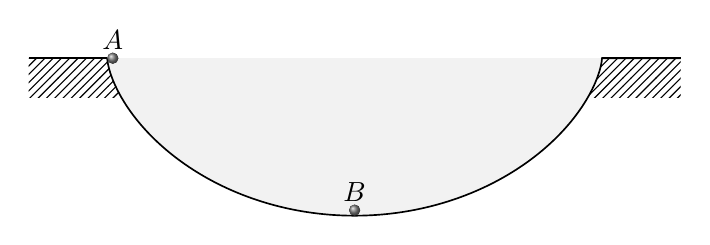
\begin{tikzpicture}[>=latex,scale=1,inner sep=1pt]
  \fill[pattern=north east lines](-1,-0.01)rectangle(1+2*pi,-.5);
  \draw[semithick](-1,0)--(0,0)(2*pi,0)--++(1,0);
  \draw[semithick,domain=0:360,samples=200,fill=lightgray!20] plot ({\x/180*pi-sin(\x)},{cos(\x)-1})--++(1,0);
  \fill[ball color=gray](pi,-2cm+2pt)circle(2pt)node[above=2pt]{$B$};
  \fill[ball color=gray](2pt,0)circle(2pt)node[above=2pt]{$A$};
\end{tikzpicture}
\end{document}